\documentclass[twoside]{book}

% Packages required by doxygen
\usepackage{fixltx2e}
\usepackage{calc}
\usepackage{doxygen}
\usepackage[export]{adjustbox} % also loads graphicx
\usepackage{graphicx}
\usepackage[utf8]{inputenc}
\usepackage{makeidx}
\usepackage{multicol}
\usepackage{multirow}
\PassOptionsToPackage{warn}{textcomp}
\usepackage{textcomp}
\usepackage[nointegrals]{wasysym}
\usepackage[table]{xcolor}

% Font selection
\usepackage[T1]{fontenc}
\usepackage[scaled=.90]{helvet}
\usepackage{courier}
\usepackage{amssymb}
\usepackage{sectsty}
\renewcommand{\familydefault}{\sfdefault}
\allsectionsfont{%
  \fontseries{bc}\selectfont%
  \color{darkgray}%
}
\renewcommand{\DoxyLabelFont}{%
  \fontseries{bc}\selectfont%
  \color{darkgray}%
}
\newcommand{\+}{\discretionary{\mbox{\scriptsize$\hookleftarrow$}}{}{}}

% Page & text layout
\usepackage{geometry}
\geometry{%
  a4paper,%
  top=2.5cm,%
  bottom=2.5cm,%
  left=2.5cm,%
  right=2.5cm%
}
\tolerance=750
\hfuzz=15pt
\hbadness=750
\setlength{\emergencystretch}{15pt}
\setlength{\parindent}{0cm}
\setlength{\parskip}{3ex plus 2ex minus 2ex}
\makeatletter
\renewcommand{\paragraph}{%
  \@startsection{paragraph}{4}{0ex}{-1.0ex}{1.0ex}{%
    \normalfont\normalsize\bfseries\SS@parafont%
  }%
}
\renewcommand{\subparagraph}{%
  \@startsection{subparagraph}{5}{0ex}{-1.0ex}{1.0ex}{%
    \normalfont\normalsize\bfseries\SS@subparafont%
  }%
}
\makeatother

% Headers & footers
\usepackage{fancyhdr}
\pagestyle{fancyplain}
\fancyhead[LE]{\fancyplain{}{\bfseries\thepage}}
\fancyhead[CE]{\fancyplain{}{}}
\fancyhead[RE]{\fancyplain{}{\bfseries\leftmark}}
\fancyhead[LO]{\fancyplain{}{\bfseries\rightmark}}
\fancyhead[CO]{\fancyplain{}{}}
\fancyhead[RO]{\fancyplain{}{\bfseries\thepage}}
\fancyfoot[LE]{\fancyplain{}{}}
\fancyfoot[CE]{\fancyplain{}{}}
\fancyfoot[RE]{\fancyplain{}{\bfseries\scriptsize Generated by Doxygen }}
\fancyfoot[LO]{\fancyplain{}{\bfseries\scriptsize Generated by Doxygen }}
\fancyfoot[CO]{\fancyplain{}{}}
\fancyfoot[RO]{\fancyplain{}{}}
\renewcommand{\footrulewidth}{0.4pt}
\renewcommand{\chaptermark}[1]{%
  \markboth{#1}{}%
}
\renewcommand{\sectionmark}[1]{%
  \markright{\thesection\ #1}%
}

% Indices & bibliography
\usepackage{natbib}
\usepackage[titles]{tocloft}
\setcounter{tocdepth}{3}
\setcounter{secnumdepth}{5}
\makeindex

% Hyperlinks (required, but should be loaded last)
\usepackage{ifpdf}
\ifpdf
  \usepackage[pdftex,pagebackref=true]{hyperref}
\else
  \usepackage[ps2pdf,pagebackref=true]{hyperref}
\fi
\hypersetup{%
  colorlinks=true,%
  linkcolor=blue,%
  citecolor=blue,%
  unicode%
}

% Custom commands
\newcommand{\clearemptydoublepage}{%
  \newpage{\pagestyle{empty}\cleardoublepage}%
}

\usepackage{caption}
\captionsetup{labelsep=space,justification=centering,font={bf},singlelinecheck=off,skip=4pt,position=top}

%===== C O N T E N T S =====

\begin{document}

% Titlepage & ToC
\hypersetup{pageanchor=false,
             bookmarksnumbered=true,
             pdfencoding=unicode
            }
\pagenumbering{alph}
\begin{titlepage}
\vspace*{7cm}
\begin{center}%
{\Large H\+H\+RM }\\
\vspace*{1cm}
{\large Generated by Doxygen 1.8.13}\\
\end{center}
\end{titlepage}
\clearemptydoublepage
\pagenumbering{roman}
\tableofcontents
\clearemptydoublepage
\pagenumbering{arabic}
\hypersetup{pageanchor=true}

%--- Begin generated contents ---
\chapter{Hierarchical Index}
\section{Class Hierarchy}
This inheritance list is sorted roughly, but not completely, alphabetically\+:\begin{DoxyCompactList}
\item \contentsline{section}{agent.\+Agent}{\pageref{classagent_1_1Agent}}{}
\item \contentsline{section}{climate\+\_\+life.\+Climate\+Life}{\pageref{classclimate__life_1_1ClimateLife}}{}
\item \contentsline{section}{hh\+\_\+register.\+H\+H\+Register}{\pageref{classhh__register_1_1HHRegister}}{}
\item Agent\begin{DoxyCompactList}
\item \contentsline{section}{government.\+Government}{\pageref{classgovernment_1_1Government}}{}
\item \contentsline{section}{household.\+Household}{\pageref{classhousehold_1_1Household}}{}
\item \contentsline{section}{shock.\+Shock}{\pageref{classshock_1_1Shock}}{}
\end{DoxyCompactList}
\end{DoxyCompactList}

\chapter{Class Index}
\section{Class List}
Here are the classes, structs, unions and interfaces with brief descriptions\+:\begin{DoxyCompactList}
\item\contentsline{section}{\hyperlink{classagent_1_1Agent}{agent.\+Agent} }{\pageref{classagent_1_1Agent}}{}
\item\contentsline{section}{\hyperlink{classclimate__life_1_1ClimateLife}{climate\+\_\+life.\+Climate\+Life} }{\pageref{classclimate__life_1_1ClimateLife}}{}
\item\contentsline{section}{\hyperlink{classgovernment_1_1Government}{government.\+Government} }{\pageref{classgovernment_1_1Government}}{}
\item\contentsline{section}{\hyperlink{classhh__register_1_1HHRegister}{hh\+\_\+register.\+H\+H\+Register} }{\pageref{classhh__register_1_1HHRegister}}{}
\item\contentsline{section}{\hyperlink{classhousehold_1_1Household}{household.\+Household} \\*\hyperlink{classhousehold_1_1Household}{Household} definition }{\pageref{classhousehold_1_1Household}}{}
\item\contentsline{section}{\hyperlink{classshock_1_1Shock}{shock.\+Shock} }{\pageref{classshock_1_1Shock}}{}
\end{DoxyCompactList}

\chapter{Class Documentation}
\hypertarget{classagent_1_1Agent}{}\section{agent.\+Agent Class Reference}
\label{classagent_1_1Agent}\index{agent.\+Agent@{agent.\+Agent}}
\subsection*{Public Member Functions}
\begin{DoxyCompactItemize}
\item 
\mbox{\Hypertarget{classagent_1_1Agent_a7ffaa2388d96a499509a7ab3a9e06a5d}\label{classagent_1_1Agent_a7ffaa2388d96a499509a7ab3a9e06a5d}} 
def {\bfseries \+\_\+\+\_\+init\+\_\+\+\_\+} (self, agent\+\_\+type)
\item 
\mbox{\Hypertarget{classagent_1_1Agent_a7e4ea84954bdb61816c715f7bd0c271d}\label{classagent_1_1Agent_a7e4ea84954bdb61816c715f7bd0c271d}} 
def {\bfseries update} (self)
\end{DoxyCompactItemize}
\subsection*{Public Attributes}
\begin{DoxyCompactItemize}
\item 
\mbox{\Hypertarget{classagent_1_1Agent_a6d3fc64fc2460eef6855e3601caec937}\label{classagent_1_1Agent_a6d3fc64fc2460eef6855e3601caec937}} 
{\bfseries agent\+\_\+type}
\end{DoxyCompactItemize}


The documentation for this class was generated from the following file\+:\begin{DoxyCompactItemize}
\item 
/home/insauer/projects/\+W\+B\+\_\+model/hhwb/hhwb/agents/agent.\+py\end{DoxyCompactItemize}

\hypertarget{classclimate__life_1_1ClimateLife}{}\section{climate\+\_\+life.\+Climate\+Life Class Reference}
\label{classclimate__life_1_1ClimateLife}\index{climate\+\_\+life.\+Climate\+Life@{climate\+\_\+life.\+Climate\+Life}}
\subsection*{Public Member Functions}
\begin{DoxyCompactItemize}
\item 
\mbox{\Hypertarget{classclimate__life_1_1ClimateLife_a587cb9ad089df966ec5582af3b256f30}\label{classclimate__life_1_1ClimateLife_a587cb9ad089df966ec5582af3b256f30}} 
def {\bfseries \+\_\+\+\_\+init\+\_\+\+\_\+} (self)
\item 
\mbox{\Hypertarget{classclimate__life_1_1ClimateLife_a4de90962fc1944e169fefaf7e64f880b}\label{classclimate__life_1_1ClimateLife_a4de90962fc1944e169fefaf7e64f880b}} 
def {\bfseries start} (self)
\end{DoxyCompactItemize}
\subsection*{Public Attributes}
\begin{DoxyCompactItemize}
\item 
\mbox{\Hypertarget{classclimate__life_1_1ClimateLife_ab6196f7fa6035efafd01e78c8f56083f}\label{classclimate__life_1_1ClimateLife_ab6196f7fa6035efafd01e78c8f56083f}} 
{\bfseries vul}
\end{DoxyCompactItemize}


The documentation for this class was generated from the following file\+:\begin{DoxyCompactItemize}
\item 
/home/insauer/projects/\+W\+B\+\_\+model/hhwb/hhwb/application/climate\+\_\+life.\+py\end{DoxyCompactItemize}

\hypertarget{classgovernment_1_1Government}{}\section{government.\+Government Class Reference}
\label{classgovernment_1_1Government}\index{government.\+Government@{government.\+Government}}


Inheritance diagram for government.\+Government\+:\nopagebreak
\begin{figure}[H]
\begin{center}
\leavevmode
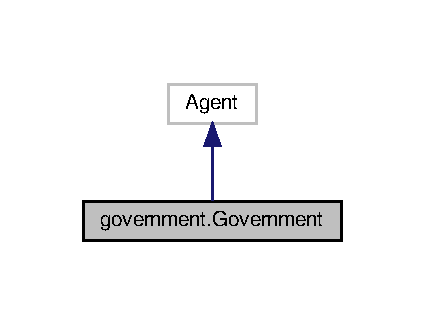
\includegraphics[width=204pt]{classgovernment_1_1Government__inherit__graph}
\end{center}
\end{figure}


Collaboration diagram for government.\+Government\+:\nopagebreak
\begin{figure}[H]
\begin{center}
\leavevmode
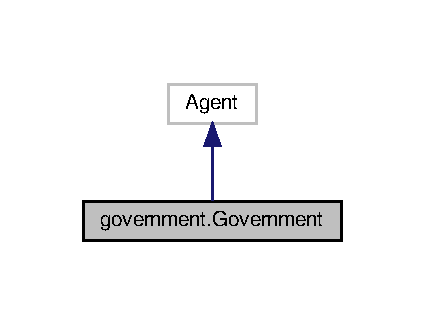
\includegraphics[width=204pt]{classgovernment_1_1Government__coll__graph}
\end{center}
\end{figure}
\subsection*{Public Member Functions}
\begin{DoxyCompactItemize}
\item 
def \hyperlink{classgovernment_1_1Government_a20d7e7f64fa8fed27b63ace640f38065}{\+\_\+\+\_\+init\+\_\+\+\_\+} (self)
\item 
\mbox{\Hypertarget{classgovernment_1_1Government_a9c46e1fc5740686cf4caabb7455242e4}\label{classgovernment_1_1Government_a9c46e1fc5740686cf4caabb7455242e4}} 
def {\bfseries tax\+\_\+rate} (self)
\item 
\mbox{\Hypertarget{classgovernment_1_1Government_a576829808c2a5fa937bfe14cdf764741}\label{classgovernment_1_1Government_a576829808c2a5fa937bfe14cdf764741}} 
def {\bfseries sp\+\_\+cost} (self)
\item 
\mbox{\Hypertarget{classgovernment_1_1Government_aac69e3171408501995df5aa8885caaa6}\label{classgovernment_1_1Government_aac69e3171408501995df5aa8885caaa6}} 
def {\bfseries K} (self)
\item 
\mbox{\Hypertarget{classgovernment_1_1Government_a2eb88be006ea8dc3d2b8ccb1130e6c71}\label{classgovernment_1_1Government_a2eb88be006ea8dc3d2b8ccb1130e6c71}} 
def {\bfseries L\+\_\+t} (self)
\item 
\mbox{\Hypertarget{classgovernment_1_1Government_a1a28cd2b1dd21cf5b8b8d384efcbe9a8}\label{classgovernment_1_1Government_a1a28cd2b1dd21cf5b8b8d384efcbe9a8}} 
def {\bfseries update} (self, hh)
\item 
def \hyperlink{classgovernment_1_1Government_adc27c11d09806596774abc2b4e786cc4}{set\+\_\+tax\+\_\+rate} (self, reg\+\_\+hh)
\item 
\mbox{\Hypertarget{classgovernment_1_1Government_ae63c718191d2781db4567e0aa30cf444}\label{classgovernment_1_1Government_ae63c718191d2781db4567e0aa30cf444}} 
def {\bfseries start\+\_\+hh\+\_\+reco} (self)
\item 
\mbox{\Hypertarget{classgovernment_1_1Government_a52f80ef2c1d974be4543e1f368e3a928}\label{classgovernment_1_1Government_a52f80ef2c1d974be4543e1f368e3a928}} 
def {\bfseries update\+\_\+\+L\+\_\+t} (self, reg\+\_\+hh)
\end{DoxyCompactItemize}


\subsection{Detailed Description}
\begin{DoxyVerb}Household definition. Computed from the FIES and interacts with the classes
Government and Shock.

Attributes:
    ***Attributes regarding the predisaster situation***
    tax_rate (float): flat income tax
    sp_cost (float): total spendings on social transfers
    K (float): Total national capital stock

    ***Attributes related to disaster recovery***
    L_0 (list): total national damage experienced at each shock
    vul (list): conceptional vulnerability at each shock as ratio L/K
    lmbda (float): optimal recovery rate
    tau (float): time at which 95% of capital stock is recovered
    L_t (float): loss at timestep t after disaster
\end{DoxyVerb}
 

\subsection{Constructor \& Destructor Documentation}
\mbox{\Hypertarget{classgovernment_1_1Government_a20d7e7f64fa8fed27b63ace640f38065}\label{classgovernment_1_1Government_a20d7e7f64fa8fed27b63ace640f38065}} 
\index{government\+::\+Government@{government\+::\+Government}!\+\_\+\+\_\+init\+\_\+\+\_\+@{\+\_\+\+\_\+init\+\_\+\+\_\+}}
\index{\+\_\+\+\_\+init\+\_\+\+\_\+@{\+\_\+\+\_\+init\+\_\+\+\_\+}!government\+::\+Government@{government\+::\+Government}}
\subsubsection{\texorpdfstring{\+\_\+\+\_\+init\+\_\+\+\_\+()}{\_\_init\_\_()}}
{\footnotesize\ttfamily def government.\+Government.\+\_\+\+\_\+init\+\_\+\+\_\+ (\begin{DoxyParamCaption}\item[{}]{self }\end{DoxyParamCaption})}

\begin{DoxyVerb}Empty Definition\end{DoxyVerb}
 

\subsection{Member Function Documentation}
\mbox{\Hypertarget{classgovernment_1_1Government_adc27c11d09806596774abc2b4e786cc4}\label{classgovernment_1_1Government_adc27c11d09806596774abc2b4e786cc4}} 
\index{government\+::\+Government@{government\+::\+Government}!set\+\_\+tax\+\_\+rate@{set\+\_\+tax\+\_\+rate}}
\index{set\+\_\+tax\+\_\+rate@{set\+\_\+tax\+\_\+rate}!government\+::\+Government@{government\+::\+Government}}
\subsubsection{\texorpdfstring{set\+\_\+tax\+\_\+rate()}{set\_tax\_rate()}}
{\footnotesize\ttfamily def government.\+Government.\+set\+\_\+tax\+\_\+rate (\begin{DoxyParamCaption}\item[{}]{self,  }\item[{}]{reg\+\_\+hh }\end{DoxyParamCaption})}

\begin{DoxyVerb}Sets the optimal tax rate basing on the total enrollment for social transfers and
extracts capital stock from each hh to get total national capital stock
    Parameters:
reg_hh (list): all registered households
\end{DoxyVerb}
 

The documentation for this class was generated from the following file\+:\begin{DoxyCompactItemize}
\item 
/home/insauer/projects/\+W\+B\+\_\+model/hhwb/hhwb/agents/government.\+py\end{DoxyCompactItemize}

\hypertarget{classhh__register_1_1HHRegister}{}\section{hh\+\_\+register.\+H\+H\+Register Class Reference}
\label{classhh__register_1_1HHRegister}\index{hh\+\_\+register.\+H\+H\+Register@{hh\+\_\+register.\+H\+H\+Register}}
\subsection*{Public Member Functions}
\begin{DoxyCompactItemize}
\item 
\mbox{\Hypertarget{classhh__register_1_1HHRegister_a347ae8c093b6e38837d200afb8ca5275}\label{classhh__register_1_1HHRegister_a347ae8c093b6e38837d200afb8ca5275}} 
def {\bfseries \+\_\+\+\_\+init\+\_\+\+\_\+} (self)
\item 
\mbox{\Hypertarget{classhh__register_1_1HHRegister_a2b0a16d9c29fbfd0e083f584ee2190fa}\label{classhh__register_1_1HHRegister_a2b0a16d9c29fbfd0e083f584ee2190fa}} 
def {\bfseries hh\+\_\+list} (self)
\item 
\mbox{\Hypertarget{classhh__register_1_1HHRegister_a53962d9da6041c5613ff84a6ceb11704}\label{classhh__register_1_1HHRegister_a53962d9da6041c5613ff84a6ceb11704}} 
def {\bfseries n\+\_\+hh} (self)
\item 
def \hyperlink{classhh__register_1_1HHRegister_ac4f13033280159722bcfbac281973465}{set\+\_\+from\+\_\+csv} (self, path=\textquotesingle{}/data/test\+\_\+data.\+csv\textquotesingle{}, id\+\_\+col=\textquotesingle{}H\+H\+ID\textquotesingle{}, weight\+\_\+col=\textquotesingle{}weight\textquotesingle{}, vul\+\_\+col=\textquotesingle{}vul\textquotesingle{}, income\+\_\+col=\textquotesingle{}income\textquotesingle{}, income\+\_\+sp=\textquotesingle{}income\+\_\+sp\textquotesingle{})
\end{DoxyCompactItemize}


\subsection{Detailed Description}
\begin{DoxyVerb}This class represents the intersection between the FIES and the model. All households
   listed in the FIES are initialised as an household object extracting information from the
   relevant columns. All required column names need to be provided during the initialisation
   of the HHRegister. The major attribute needed for further modeling is then a list of all
   registered households.

   Attributes:

       hh_list (list): list with the registered households
       n_hh (int): number of registered households
\end{DoxyVerb}
 

\subsection{Member Function Documentation}
\mbox{\Hypertarget{classhh__register_1_1HHRegister_ac4f13033280159722bcfbac281973465}\label{classhh__register_1_1HHRegister_ac4f13033280159722bcfbac281973465}} 
\index{hh\+\_\+register\+::\+H\+H\+Register@{hh\+\_\+register\+::\+H\+H\+Register}!set\+\_\+from\+\_\+csv@{set\+\_\+from\+\_\+csv}}
\index{set\+\_\+from\+\_\+csv@{set\+\_\+from\+\_\+csv}!hh\+\_\+register\+::\+H\+H\+Register@{hh\+\_\+register\+::\+H\+H\+Register}}
\subsubsection{\texorpdfstring{set\+\_\+from\+\_\+csv()}{set\_from\_csv()}}
{\footnotesize\ttfamily def hh\+\_\+register.\+H\+H\+Register.\+set\+\_\+from\+\_\+csv (\begin{DoxyParamCaption}\item[{}]{self,  }\item[{}]{path = {\ttfamily \textquotesingle{}/data/test\+\_\+data.csv\textquotesingle{}},  }\item[{}]{id\+\_\+col = {\ttfamily \textquotesingle{}HHID\textquotesingle{}},  }\item[{}]{weight\+\_\+col = {\ttfamily \textquotesingle{}weight\textquotesingle{}},  }\item[{}]{vul\+\_\+col = {\ttfamily \textquotesingle{}vul\textquotesingle{}},  }\item[{}]{income\+\_\+col = {\ttfamily \textquotesingle{}income\textquotesingle{}},  }\item[{}]{income\+\_\+sp = {\ttfamily \textquotesingle{}income\+\_\+sp\textquotesingle{}} }\end{DoxyParamCaption})}

\begin{DoxyVerb}This function reads the household information from the FIES if it is given in a
csv file. It provides the full list of household agents.

Parameters:
    path (str): path of the input data frame
    id_col (str): column name of the column containing the household ID
    income_col (str): column name of the column containing the household's total income
    income_sp (str): column name of the column containing the household's income from
              social transfers
    weight_col (str): column name of the column containing the household's weightinc_reco
    vul_col (str): column name of the column containing the household's vulnerability
\end{DoxyVerb}
 

The documentation for this class was generated from the following file\+:\begin{DoxyCompactItemize}
\item 
/home/insauer/projects/\+W\+B\+\_\+model/hhwb/hhwb/agents/hh\+\_\+register.\+py\end{DoxyCompactItemize}

\hypertarget{classhousehold_1_1Household}{}\section{household.\+Household Class Reference}
\label{classhousehold_1_1Household}\index{household.\+Household@{household.\+Household}}


\hyperlink{classhousehold_1_1Household}{Household} definition.  




Inheritance diagram for household.\+Household\+:\nopagebreak
\begin{figure}[H]
\begin{center}
\leavevmode
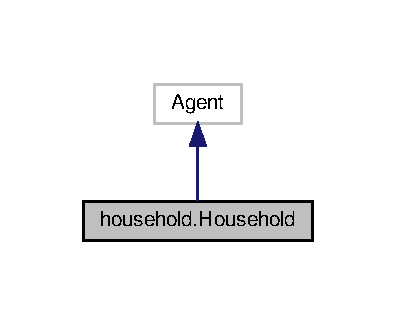
\includegraphics[width=190pt]{classhousehold_1_1Household__inherit__graph}
\end{center}
\end{figure}


Collaboration diagram for household.\+Household\+:\nopagebreak
\begin{figure}[H]
\begin{center}
\leavevmode
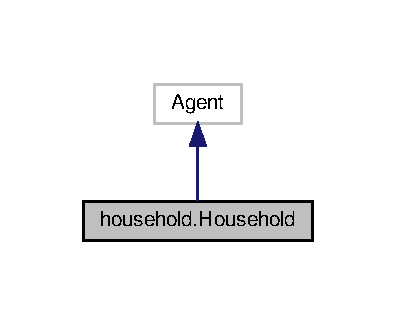
\includegraphics[width=190pt]{classhousehold_1_1Household__coll__graph}
\end{center}
\end{figure}
\subsection*{Public Member Functions}
\begin{DoxyCompactItemize}
\item 
\mbox{\Hypertarget{classhousehold_1_1Household_aed0855bd50448e9bc536630f16daa2b3}\label{classhousehold_1_1Household_aed0855bd50448e9bc536630f16daa2b3}} 
def \hyperlink{classhousehold_1_1Household_aed0855bd50448e9bc536630f16daa2b3}{\+\_\+\+\_\+init\+\_\+\+\_\+} (self, hhid=0, w=1., vul=0.\+2, i\+\_\+0=1., i\+\_\+sp=0.\+2)
\begin{DoxyCompactList}\small\item\em constructor \end{DoxyCompactList}\item 
\mbox{\Hypertarget{classhousehold_1_1Household_aabaf41441c901535463af6fca80e3a4a}\label{classhousehold_1_1Household_aabaf41441c901535463af6fca80e3a4a}} 
def {\bfseries hhid} (self)
\item 
\mbox{\Hypertarget{classhousehold_1_1Household_afa93ee191a65e945a4200a203966cd00}\label{classhousehold_1_1Household_afa93ee191a65e945a4200a203966cd00}} 
def {\bfseries weight} (self)
\item 
\mbox{\Hypertarget{classhousehold_1_1Household_ac9195196e8eb6a01ff7257e66777f52b}\label{classhousehold_1_1Household_ac9195196e8eb6a01ff7257e66777f52b}} 
def {\bfseries affected} (self)
\item 
\mbox{\Hypertarget{classhousehold_1_1Household_ab6869bf2e80c8c232825092c39679f6b}\label{classhousehold_1_1Household_ab6869bf2e80c8c232825092c39679f6b}} 
def {\bfseries d\+\_\+k\+\_\+eff\+\_\+t} (self)
\item 
\mbox{\Hypertarget{classhousehold_1_1Household_a7c1a7145a13b716175bbade3b1c590d4}\label{classhousehold_1_1Household_a7c1a7145a13b716175bbade3b1c590d4}} 
def {\bfseries lmbda} (self)
\item 
\mbox{\Hypertarget{classhousehold_1_1Household_a84f840e4f5e8e2283f62a952384c6808}\label{classhousehold_1_1Household_a84f840e4f5e8e2283f62a952384c6808}} 
def {\bfseries vul} (self)
\item 
\mbox{\Hypertarget{classhousehold_1_1Household_a2e841d098af926fafc5a27af890fe200}\label{classhousehold_1_1Household_a2e841d098af926fafc5a27af890fe200}} 
def {\bfseries tau} (self)
\item 
\mbox{\Hypertarget{classhousehold_1_1Household_a82ed796b45f048ebbc8f716226810cc9}\label{classhousehold_1_1Household_a82ed796b45f048ebbc8f716226810cc9}} 
def {\bfseries income\+\_\+0} (self)
\item 
\mbox{\Hypertarget{classhousehold_1_1Household_aa19eaf3597895e341df0d6a43a96edcb}\label{classhousehold_1_1Household_aa19eaf3597895e341df0d6a43a96edcb}} 
def {\bfseries income\+\_\+sp} (self)
\item 
\mbox{\Hypertarget{classhousehold_1_1Household_a3ebcba1436e6a10122ad7e4ce91a1cb8}\label{classhousehold_1_1Household_a3ebcba1436e6a10122ad7e4ce91a1cb8}} 
def {\bfseries consum\+\_\+0} (self)
\item 
\mbox{\Hypertarget{classhousehold_1_1Household_a5e3dae2dc76d3d57f5b8730502595db7}\label{classhousehold_1_1Household_a5e3dae2dc76d3d57f5b8730502595db7}} 
def {\bfseries d\+\_\+inc\+\_\+t} (self)
\item 
\mbox{\Hypertarget{classhousehold_1_1Household_a9613c8f8f2e2a44b76f6ac963989cec0}\label{classhousehold_1_1Household_a9613c8f8f2e2a44b76f6ac963989cec0}} 
def {\bfseries d\+\_\+inc\+\_\+sp\+\_\+t} (self)
\item 
\mbox{\Hypertarget{classhousehold_1_1Household_a477e6eb34e1fd715e588f01574933807}\label{classhousehold_1_1Household_a477e6eb34e1fd715e588f01574933807}} 
def {\bfseries d\+\_\+con\+\_\+t} (self)
\item 
\mbox{\Hypertarget{classhousehold_1_1Household_a27179fc4eb8626534a05ebe4e0f4a065}\label{classhousehold_1_1Household_a27179fc4eb8626534a05ebe4e0f4a065}} 
def {\bfseries k\+\_\+eff\+\_\+0} (self)
\item 
\mbox{\Hypertarget{classhousehold_1_1Household_a1957910933a58e7009dd810c12758d81}\label{classhousehold_1_1Household_a1957910933a58e7009dd810c12758d81}} 
def {\bfseries inc\+\_\+reco} (self)
\item 
\mbox{\Hypertarget{classhousehold_1_1Household_a523f19ebeabdcd3c57cb9bb65a334309}\label{classhousehold_1_1Household_a523f19ebeabdcd3c57cb9bb65a334309}} 
def {\bfseries inc\+\_\+sp\+\_\+reco} (self)
\item 
\mbox{\Hypertarget{classhousehold_1_1Household_a0a77ccddd4485b9c219b85941289a614}\label{classhousehold_1_1Household_a0a77ccddd4485b9c219b85941289a614}} 
def {\bfseries cons\+\_\+reco} (self)
\item 
\mbox{\Hypertarget{classhousehold_1_1Household_a0ca97ee6f389f5f13f213c9d46b304be}\label{classhousehold_1_1Household_a0ca97ee6f389f5f13f213c9d46b304be}} 
def {\bfseries k\+\_\+eff\+\_\+reco} (self)
\item 
\mbox{\Hypertarget{classhousehold_1_1Household_a53127e2b912ecfce7ed0cdb8119ecf9f}\label{classhousehold_1_1Household_a53127e2b912ecfce7ed0cdb8119ecf9f}} 
def {\bfseries set\+\_\+tax\+\_\+rate} (self, tax\+\_\+rate=0)
\item 
def \hyperlink{classhousehold_1_1Household_af60008bacefd13fc398091bc7fc06f05}{init\+\_\+reco} (self)
\item 
def \hyperlink{classhousehold_1_1Household_a96a14035a0b3c03c6cf951251d5f941e}{update\+\_\+reco} (self, t, t\+\_\+i, L\+\_\+t, K)
\item 
def \hyperlink{classhousehold_1_1Household_ab9aa47f8e64ddaf4825c90c1832b3ddd}{shock} (self, reco\+\_\+period=R\+E\+C\+O\+\_\+\+P\+E\+R\+I\+OD, temp\+\_\+res=T\+E\+M\+P\+\_\+\+R\+ES, aff\+\_\+flag=False, L=0, K=0)
\item 
\mbox{\Hypertarget{classhousehold_1_1Household_ad17bac4d94f85674706a38d75f49cf5f}\label{classhousehold_1_1Household_ad17bac4d94f85674706a38d75f49cf5f}} 
def {\bfseries set\+\_\+k\+\_\+eff\+\_\+0} (self)
\item 
\mbox{\Hypertarget{classhousehold_1_1Household_ae27f3f5fc9f5aedd97ebd5893b9fe08d}\label{classhousehold_1_1Household_ae27f3f5fc9f5aedd97ebd5893b9fe08d}} 
def {\bfseries plot\+\_\+reco\+\_\+trajec} (self, timeframe=40, pred=5)
\item 
\mbox{\Hypertarget{classhousehold_1_1Household_acfc35999faf730815e06efcb2ad28bfe}\label{classhousehold_1_1Household_acfc35999faf730815e06efcb2ad28bfe}} 
def {\bfseries plot\+\_\+life\+\_\+trajec} (self, timeframe=40, pred=5)
\end{DoxyCompactItemize}


\subsection{Detailed Description}
\hyperlink{classhousehold_1_1Household}{Household} definition. 

Computed from the F\+I\+ES and interacts with the classes Government and Shock. Attributes\+: 
\begin{DoxyParams}{Parameters}
{\em hhid} & (int)\+: household id \\
\hline
{\em weight} & (float)\+: household weight (summing up over all household weights returns the total population of the administrative unit) \\
\hline
{\em vul} & (float)\+: household vulnerability (independent of disaster magnitude) \\
\hline
{\em inc\+\_\+0} & (float)\+: Total income in the predisaster situation \\
\hline
{\em inc\+\_\+sp} & (float)\+: Total income from social transfers in the predisaster situation \\
\hline
{\em con\+\_\+0} & predisaster consumption\\
\hline
\end{DoxyParams}
{\itshape {\bfseries Attributes calculated for the predisaster situation (F\+I\+ES) and national indicators}} 
\begin{DoxyParams}{Parameters}
{\em k\+\_\+eff\+\_\+0} & predisaster effective capital stock \\
\hline
{\em lmbda} & optimal reconstruction rate \\
\hline
{\em tau} & time needed to achieve 95\% recovery\\
\hline
\end{DoxyParams}
{\itshape {\bfseries Attributes related to disaster recovery}} 
\begin{DoxyParams}{Parameters}
{\em ff} & (list)\+: bools showing whether the household was affected by a shock or not \\
\hline
{\em damage} & (list)\+: Experienced direct damage at each event \\
\hline
{\em d\+\_\+k\+\_\+eff\+\_\+t} & (float)\+: loss of effective capital stock at time step t after disaster \\
\hline
{\em d\+\_\+inc\+\_\+t} & (float)\+: loss of income at timestemp t \\
\hline
{\em d\+\_\+inc\+\_\+sp\+\_\+t} & (float)\+: change in income from social transfers at time step t after disaster \\
\hline
{\em d\+\_\+con\+\_\+t} & (float)\+: loss in consumption at time step t after disaster \\
\hline
{\em k\+\_\+eff\+\_\+reco} & (np.\+array)\+: recovery track of capital stock \\
\hline
{\em inc\+\_\+reco} & (np.\+array)\+: recovery track of income \\
\hline
{\em inc\+\_\+sp\+\_\+reco} & (np.\+array)\+: recovery track of income \\
\hline
{\em con\+\_\+reco} & (np.\+array)\+: recovery track of consumption \\
\hline
{\em wbls} & (float)\+: aggregated wellbeing loss \\
\hline
\end{DoxyParams}


\subsection{Member Function Documentation}
\mbox{\Hypertarget{classhousehold_1_1Household_af60008bacefd13fc398091bc7fc06f05}\label{classhousehold_1_1Household_af60008bacefd13fc398091bc7fc06f05}} 
\index{household\+::\+Household@{household\+::\+Household}!init\+\_\+reco@{init\+\_\+reco}}
\index{init\+\_\+reco@{init\+\_\+reco}!household\+::\+Household@{household\+::\+Household}}
\subsubsection{\texorpdfstring{init\+\_\+reco()}{init\_reco()}}
{\footnotesize\ttfamily def household.\+Household.\+init\+\_\+reco (\begin{DoxyParamCaption}\item[{}]{self }\end{DoxyParamCaption})}

\begin{DoxyVerb}Prepares the recovery process by calculating the household's effective capital stock and
the optimal recovery track.
\end{DoxyVerb}
 Here is the call graph for this function\+:\nopagebreak
\begin{figure}[H]
\begin{center}
\leavevmode
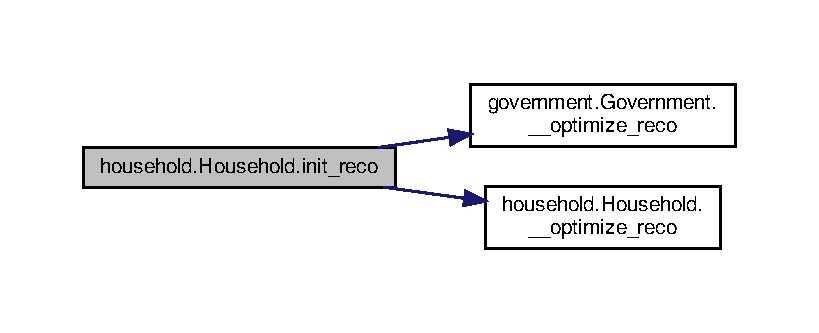
\includegraphics[width=350pt]{classhousehold_1_1Household_af60008bacefd13fc398091bc7fc06f05_cgraph}
\end{center}
\end{figure}
\mbox{\Hypertarget{classhousehold_1_1Household_ab9aa47f8e64ddaf4825c90c1832b3ddd}\label{classhousehold_1_1Household_ab9aa47f8e64ddaf4825c90c1832b3ddd}} 
\index{household\+::\+Household@{household\+::\+Household}!shock@{shock}}
\index{shock@{shock}!household\+::\+Household@{household\+::\+Household}}
\subsubsection{\texorpdfstring{shock()}{shock()}}
{\footnotesize\ttfamily def household.\+Household.\+shock (\begin{DoxyParamCaption}\item[{}]{self,  }\item[{}]{reco\+\_\+period = {\ttfamily RECO\+\_\+PERIOD},  }\item[{}]{temp\+\_\+res = {\ttfamily TEMP\+\_\+RES},  }\item[{}]{aff\+\_\+flag = {\ttfamily False},  }\item[{}]{L = {\ttfamily 0},  }\item[{}]{K = {\ttfamily 0} }\end{DoxyParamCaption})}

\begin{DoxyVerb}This function causes the household to be shocked. The recovery track is set up and the
   post disaster state is generated for all indicators.
Parameters
----------
reco_period : int, optional
    Time frame after first disaster in years where reconstruction is modeled (in years).
    The default is RECO_PERIOD.
temp_res : TYPE, optional
    Temporal resolution after recovery in weeks. The default is TEMP_RES.
aff_flag : bool, optional
    Bool indicating whether the household is affected by the current shock.
    The default is False.
L : float, optional
    Total national damage. The default is 0.
K : float, optional
    Total national capital stock. The default is 0.
\end{DoxyVerb}
 Here is the call graph for this function\+:\nopagebreak
\begin{figure}[H]
\begin{center}
\leavevmode
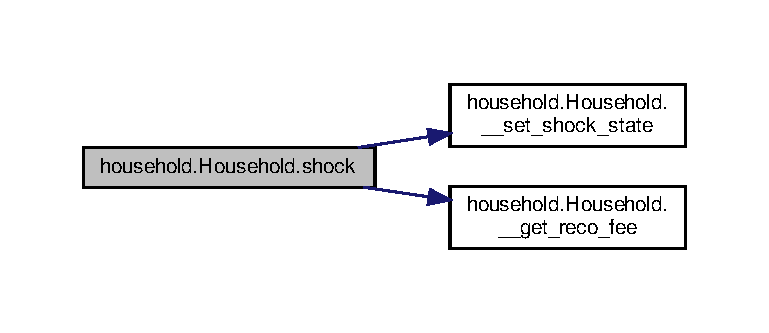
\includegraphics[width=350pt]{classhousehold_1_1Household_ab9aa47f8e64ddaf4825c90c1832b3ddd_cgraph}
\end{center}
\end{figure}
\mbox{\Hypertarget{classhousehold_1_1Household_a96a14035a0b3c03c6cf951251d5f941e}\label{classhousehold_1_1Household_a96a14035a0b3c03c6cf951251d5f941e}} 
\index{household\+::\+Household@{household\+::\+Household}!update\+\_\+reco@{update\+\_\+reco}}
\index{update\+\_\+reco@{update\+\_\+reco}!household\+::\+Household@{household\+::\+Household}}
\subsubsection{\texorpdfstring{update\+\_\+reco()}{update\_reco()}}
{\footnotesize\ttfamily def household.\+Household.\+update\+\_\+reco (\begin{DoxyParamCaption}\item[{}]{self,  }\item[{}]{t,  }\item[{}]{t\+\_\+i,  }\item[{}]{L\+\_\+t,  }\item[{}]{K }\end{DoxyParamCaption})}

\begin{DoxyVerb}Parameters
----------
t : TYPE
    DESCRIPTION.
t_i : TYPE
    DESCRIPTION.
L_t : TYPE
    DESCRIPTION.
K : TYPE
    DESCRIPTION.

Returns
-------
None.\end{DoxyVerb}
 Here is the call graph for this function\+:\nopagebreak
\begin{figure}[H]
\begin{center}
\leavevmode
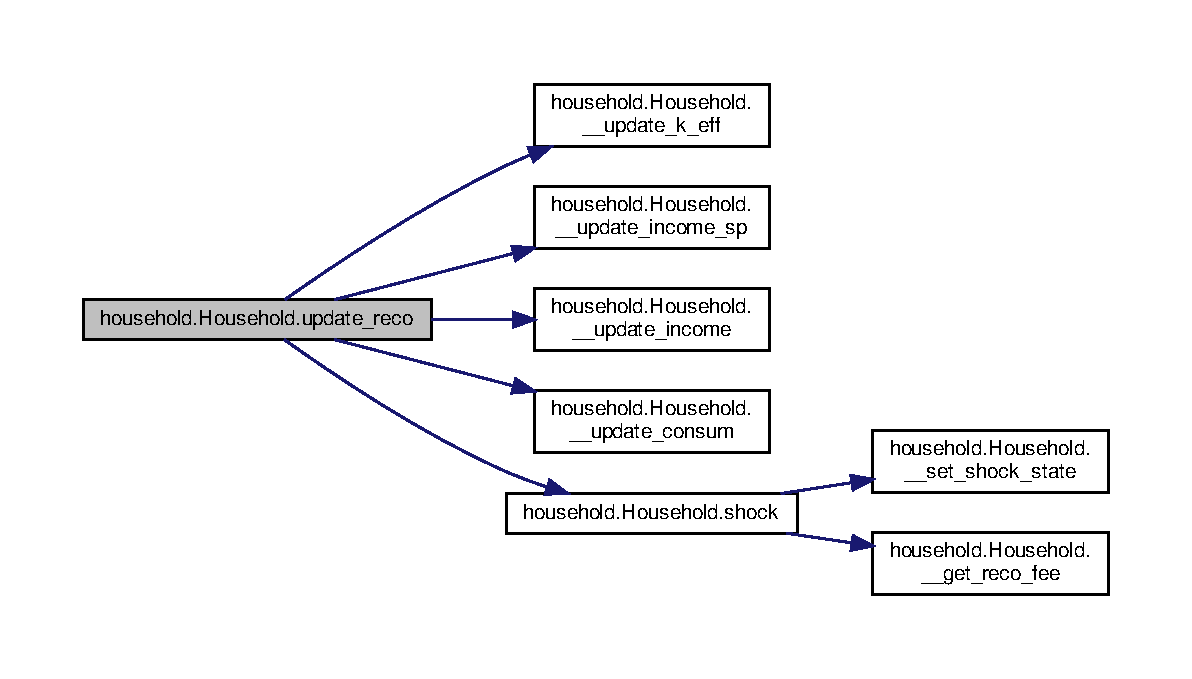
\includegraphics[width=350pt]{classhousehold_1_1Household_a96a14035a0b3c03c6cf951251d5f941e_cgraph}
\end{center}
\end{figure}


The documentation for this class was generated from the following file\+:\begin{DoxyCompactItemize}
\item 
/home/insauer/projects/\+W\+B\+\_\+model/hhwb/hhwb/agents/household.\+py\end{DoxyCompactItemize}

\hypertarget{classshock_1_1Shock}{}\section{shock.\+Shock Class Reference}
\label{classshock_1_1Shock}\index{shock.\+Shock@{shock.\+Shock}}


Inheritance diagram for shock.\+Shock\+:\nopagebreak
\begin{figure}[H]
\begin{center}
\leavevmode
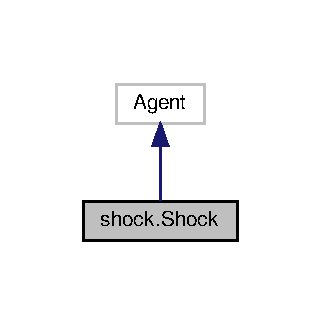
\includegraphics[width=154pt]{classshock_1_1Shock__inherit__graph}
\end{center}
\end{figure}


Collaboration diagram for shock.\+Shock\+:\nopagebreak
\begin{figure}[H]
\begin{center}
\leavevmode
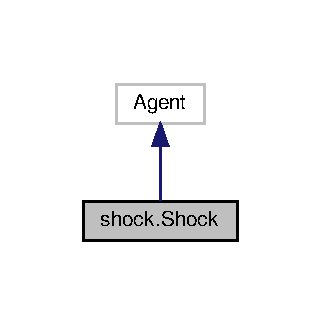
\includegraphics[width=154pt]{classshock_1_1Shock__coll__graph}
\end{center}
\end{figure}
\subsection*{Public Member Functions}
\begin{DoxyCompactItemize}
\item 
\mbox{\Hypertarget{classshock_1_1Shock_a8329cfbad2da6ad2115358a1fb1eb285}\label{classshock_1_1Shock_a8329cfbad2da6ad2115358a1fb1eb285}} 
def {\bfseries \+\_\+\+\_\+init\+\_\+\+\_\+} (self)
\item 
\mbox{\Hypertarget{classshock_1_1Shock_aeebc7c69f51fd5d99df7e54c5e00d1f8}\label{classshock_1_1Shock_aeebc7c69f51fd5d99df7e54c5e00d1f8}} 
def {\bfseries aff\+\_\+hh} (self)
\item 
\mbox{\Hypertarget{classshock_1_1Shock_a3f1238f3185a86b3bcbb0c6495a8d0d5}\label{classshock_1_1Shock_a3f1238f3185a86b3bcbb0c6495a8d0d5}} 
def {\bfseries unaff\+\_\+hh} (self)
\item 
\mbox{\Hypertarget{classshock_1_1Shock_a7db59427cbb975613758801593490a70}\label{classshock_1_1Shock_a7db59427cbb975613758801593490a70}} 
def {\bfseries L} (self)
\item 
\mbox{\Hypertarget{classshock_1_1Shock_a36753432928f5b31e8527338abad17d8}\label{classshock_1_1Shock_a36753432928f5b31e8527338abad17d8}} 
def {\bfseries dt} (self)
\item 
def \hyperlink{classshock_1_1Shock_ae3e6312bb8b5bc7962d9180ed3f17aa3}{set\+\_\+random\+\_\+shock} (self, hhs)
\item 
def \hyperlink{classshock_1_1Shock_aefe691acc8ddd7e1c42a70e529ce192f}{shock} (self, gov, hhs)
\end{DoxyCompactItemize}


\subsection{Detailed Description}
\begin{DoxyVerb}Shock definition. This class builds the intersection with Climada and provides direct
   damage obtained from Climada and the affected households.

    Attributes:
        aff_hh (list): list with affected households
        unaff_hh (list): list with uneffected households
        aff_hh_id (list): list with IDs of affected households
        unaff_hh_id (list): list with IDs of unaffected households
        L (float): total damage
\end{DoxyVerb}
 

\subsection{Member Function Documentation}
\mbox{\Hypertarget{classshock_1_1Shock_ae3e6312bb8b5bc7962d9180ed3f17aa3}\label{classshock_1_1Shock_ae3e6312bb8b5bc7962d9180ed3f17aa3}} 
\index{shock\+::\+Shock@{shock\+::\+Shock}!set\+\_\+random\+\_\+shock@{set\+\_\+random\+\_\+shock}}
\index{set\+\_\+random\+\_\+shock@{set\+\_\+random\+\_\+shock}!shock\+::\+Shock@{shock\+::\+Shock}}
\subsubsection{\texorpdfstring{set\+\_\+random\+\_\+shock()}{set\_random\_shock()}}
{\footnotesize\ttfamily def shock.\+Shock.\+set\+\_\+random\+\_\+shock (\begin{DoxyParamCaption}\item[{}]{self,  }\item[{}]{hhs }\end{DoxyParamCaption})}

\begin{DoxyVerb}The function selects households randomly and shocks them. (Function is only a
   placeholder for a real Climade intersection.

    Parameters
    ----------
    hhs : list
list with all households
\end{DoxyVerb}
 \mbox{\Hypertarget{classshock_1_1Shock_aefe691acc8ddd7e1c42a70e529ce192f}\label{classshock_1_1Shock_aefe691acc8ddd7e1c42a70e529ce192f}} 
\index{shock\+::\+Shock@{shock\+::\+Shock}!shock@{shock}}
\index{shock@{shock}!shock\+::\+Shock@{shock\+::\+Shock}}
\subsubsection{\texorpdfstring{shock()}{shock()}}
{\footnotesize\ttfamily def shock.\+Shock.\+shock (\begin{DoxyParamCaption}\item[{}]{self,  }\item[{}]{gov,  }\item[{}]{hhs }\end{DoxyParamCaption})}

\begin{DoxyVerb}The function selects households randomly and shocks them. (Function is only a
   placeholder for a real Climade intersection.

    Parameters
    ----------
    gov : Government
the government of all households
\end{DoxyVerb}
 Here is the call graph for this function\+:\nopagebreak
\begin{figure}[H]
\begin{center}
\leavevmode
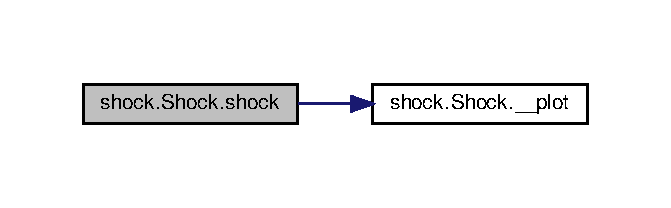
\includegraphics[width=322pt]{classshock_1_1Shock_aefe691acc8ddd7e1c42a70e529ce192f_cgraph}
\end{center}
\end{figure}


The documentation for this class was generated from the following file\+:\begin{DoxyCompactItemize}
\item 
/home/insauer/projects/\+W\+B\+\_\+model/hhwb/hhwb/agents/shock.\+py\end{DoxyCompactItemize}

%--- End generated contents ---

% Index
\backmatter
\newpage
\phantomsection
\clearemptydoublepage
\addcontentsline{toc}{chapter}{Index}
\printindex

\end{document}
